\documentclass[a4paper,14pt]{extarticle}

\usepackage[utf8x]{inputenc}
\usepackage[T1,T2A]{fontenc}
\usepackage[russian]{babel}
\usepackage{hyperref}
\usepackage{indentfirst}
\usepackage{here}
\usepackage{array}
\usepackage{graphicx}
\usepackage{caption}
\usepackage{subcaption}
\usepackage{chngcntr}
\usepackage{amsmath}
\usepackage{amssymb}
\usepackage{pgfplots}
\usepackage{pgfplotstable}
\usepackage[left=2cm,right=2cm,top=2cm,bottom=2cm,bindingoffset=0cm]{geometry}
\usepackage{multicol}

\renewcommand{\le}{\ensuremath{\leqslant}}
\renewcommand{\leq}{\ensuremath{\leqslant}}
\renewcommand{\ge}{\ensuremath{\geqslant}}
\renewcommand{\geq}{\ensuremath{\geqslant}}
\renewcommand{\epsilon}{\ensuremath{\varepsilon}}
\renewcommand{\phi}{\ensuremath{\varphi}}

\counterwithin{figure}{section}
\counterwithin{equation}{section}
\counterwithin{table}{section}
\newcommand{\sign}[1][5cm]{\makebox[#1]{\hrulefill}} % Поля подписи и даты
\graphicspath{{pics/}} % Путь до папки с картинками
\captionsetup{justification=centering,margin=1cm}
\def\arraystretch{1.3}

\usepackage{courier}

\usepackage{listings}
\lstset{ %
extendedchars=\true,
keepspaces=true,
language=C,						% choose the language of the code
basicstyle=\footnotesize,		% the size of the fonts that are used for the code
numbers=left,					% where to put the line-numbers
numberstyle=\footnotesize,		% the size of the fonts that are used for the line-numbers
stepnumber=1,					% the step between two line-numbers. If it is 1 each line will be numbered
numbersep=5pt,					% how far the line-numbers are from the code
backgroundcolor=\color{white},	% choose the background color. You must add \usepackage{color}
showspaces=false				% show spaces adding particular underscores
showstringspaces=false,			% underline spaces within strings
showtabs=false,					% show tabs within strings adding particular underscores
frame=single,           		% adds a frame around the code
tabsize=2,						% sets default tabsize to 2 spaces
captionpos=b,					% sets the caption-position to bottom
breaklines=true,				% sets automatic line breaking
breakatwhitespace=false,		% sets if automatic breaks should only happen at whitespace
escapeinside={\%*}{*)},			% if you want to add a comment within your code
postbreak=\raisebox{0ex}[0ex][0ex]{\ensuremath{\color{red}\hookrightarrow\space}},
texcl=true,
}

\lstset{basicstyle=\footnotesize\ttfamily,breaklines=true}

\begin{document}

\begin{titlepage}
\begin{center}
	\textbf{Санкт-Петербургский Политехнический Университет \\Петра Великого}\\[0.3cm]
	\small Институт компьютерных наук и технологий \\[0.3cm]
	\small Кафедра компьютерных систем и программных технологий\\[4cm]
	
	\textbf{ОТЧЕТ}\\ \textbf{о лабораторной работе}\\[0.5cm]
	\textbf{<<Использование стандартных подпрограмм для приближенного\\ вычисления интеграла>>}\\[0.1cm]
	\textbf{Вычислительная математика}\\[8.0cm]
\end{center}

\begin{flushright}
	\begin{minipage}{0.48\textwidth}
		\begin{flushleft}
			\small \textbf{Работу выполнил студент}\\[3mm]
			\small группа 23501/4 \hspace*{6mm} Дьячков В.В.\\[5mm]
			
			\small \textbf{Преподаватель}\\[5mm]
		 	\small \sign[3cm] \hspace*{5mm} к.т.н., доц. Цыган В.Н.\\[0.5cm]
		\end{flushleft}
	\end{minipage}
\end{flushright}

\vfill

\begin{center}
	\small Санкт-Петербург\\
	\small \the\year
\end{center}
\end{titlepage}

\section{Техническое задание}

\textbf{Вариант 5:} Привесети дифференциальное уравнение к системе двух дифференциальных уравнений первого порядка. Решить с шагом $h = 0.1$:
\begin{enumerate}
\item Используя подпрограмму \textbf{RKF45};
\item Используя усовершенствованный метод ломанных Эйлера.
\end{enumerate}
Сравнить результаты, полученные двумя методами, с точным решением. 

\section{Исходные данные}

Дифференциальное уравнение:
\[
t^2\cdot y'' - 12y = 0
\]

Начальные условия:
\begin{center}
\begin{multicols}{3} 
	$\left. y \right|_{t=1} = 1;$ \\
	$\left. y' \right|_{t=1} = 4;$ \\
	$1 \le t \le 2$
\end{multicols}
\end{center}

Точное решение:
\[
y(t) = t^4
\]

\section{Выполнение работы}

Исходное дифференциальное с помощью подстановок $x_1(t) = y(t)$ и $x_2(t) = y'(t)$ было приведено к системе дифференциальных уравнений первого порядка:
\[
\begin{pmatrix}
    x'_1(t) \\
    x'_2(t) \\
\end{pmatrix}
  =
\begin{pmatrix}
    0 & 1 \\
    \frac{12}{t^2} & 0 \\
\end{pmatrix}
\cdot
\begin{pmatrix}
    x_1(t) \\
    x_2(t) \\
\end{pmatrix}
\]

\vspace{0.25cm}

После чего на языке \textbf{C++} была разработана программа для решения поставленных задач (см. листинги \ref{code:mainh} и \ref{code:maincpp}). Сначала было найдено решение дифференциального уравнения помощью подпрограммы \textbf{RKF45}. Из рисунков \ref{fig:exact} и \ref{fig:rkf} видно, что полученное решение полностью совпало с точным решением.

Затем была разработана подпрограмма, находящая решение с использованием усовершенствованного метода ломанных Эйлера (см. листинги \ref{code:impeulerh} и \ref{code:impeulercpp}). Данный метод предусматривает следующий рекуррентный алгоритм: 

\[
\begin{cases}
	x_{n+1/2}^{*} = x_n + \frac{h}{2} f(t_n, x_n)
	\\
	x_{n+1} = x_n + h \left(t_n + \frac{h}{2}, x_{n+1/2}^{*} \right)
\end{cases}
\]

Из вывода программы на рисунках \ref{fig:euler} и \ref{fig:euler_error} видно, что решение, найденное данным методом оказалось гораздо менее точным, по сравнению с методом, используемым в подпрограмме \textbf{RKF45}: данное решение имеет точность менее 3 знаков после запятой. Данный факт можно объяснить тем, что усовершествованный метод ломанных Эйлера имеет вторую степень точности, в то время как метод Рунге--Кутта--Фельберга, используемый в подпрогрмме \textbf{RKF45}, обладает четвертой и пятой степенью точности.

\begin{figure}[H]
\begin{center}
	\begin{subfigure}[t]{0.35\textwidth}
		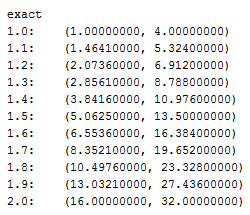
\includegraphics[scale=0.83]{exact}
		\caption{Точное решение уравнения}
		\label{fig:exact}
	\end{subfigure}
	\begin{subfigure}[t]{0.35\textwidth}
		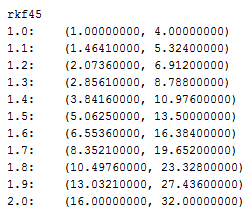
\includegraphics[scale=0.83]{rkf}
		\caption{Решение, полученное подпрограммой \texttt{RKF45}}
		\label{fig:rkf}
	\end{subfigure}
	\begin{subfigure}[t]{0.35\textwidth}
		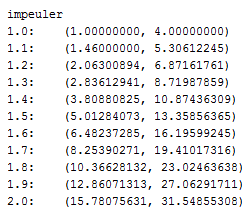
\includegraphics[scale=0.83]{euler}
		\caption{Решение, полученное усовршенствованным методом ломанных Эйлера}
		\label{fig:euler}
	\end{subfigure}
	\begin{subfigure}[t]{0.35\textwidth}
		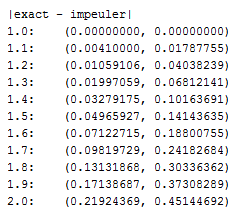
\includegraphics[scale=0.83]{euler_error}
		\caption{Погрешность полученного решения}
		\label{fig:euler_error}
	\end{subfigure}
	\caption{}
	\vspace{-0.8cm}
\end{center}
\end{figure}

На рисунке \ref{plot:solution} изображены точное решение и решение, полученное с использованием усовершенствованного метода ломанных Эйлера.

\vspace{-0.5cm}

\begin{figure}[H]
\begin{center}
	\begin{tikzpicture} [every plot/.append style={thick}]
		\begin{axis}[
			height=0.35\textheight,
			width=0.85\textwidth,
			legend pos=north west,
			xlabel={$t$},
			ylabel={$y(t)$},
			xlabel near ticks,
			ylabel near ticks,
			xmin=0.9,
			xmax=2.1,
			ymin=0,
			ymax=18,
			grid=major
		]
		\addplot table[x=t,y=x1,col sep=comma]{data/exact.csv};
		\addplot table[x=t,y=x1,col sep=comma]{data/euler.csv};
		\legend{Точное решение, Усовершествованный метод Эйлера}
		\end{axis}
	\end{tikzpicture}
	\caption{Зависимость $y$ от $t$ для точного решения и решения, полученного усовершествованным методом Эйлера}
	\label{plot:solution}
\end{center}
\end{figure}

На рисунке \ref{plot:euler_error} изображена погрешность, полученная при вычислении решения с использованием усовершенствованного метода ломанных Эйлера. Как видно, на всем промежутке $[1, 2]$ погрешность монотонно нелинейно возрастает, что объясняется накоплением глобальной погрешности.

\begin{figure}[H]
\begin{center}
	\begin{tikzpicture} [every plot/.append style={thick}]
		\begin{axis}[
			y tick label style={
				/pgf/number format/.cd,
            	fixed,
            	fixed zerofill,
            	precision=2,
        		/tikz/.cd
    		},
			height=0.35\textheight,
			width=0.85\textwidth,
			xlabel={$t$},
			ylabel={$|\epsilon(t)|$},
			xlabel near ticks,
			ylabel near ticks,
			xmin=0.9,
			xmax=2.1,
			ymin=-0.05,
			ymax=0.25,
			grid=major
		]
		\addplot table[x=t,y=x1,col sep=comma]{data/euler_error.csv};
		\end{axis}
	\end{tikzpicture}
	\caption{Зависимость погрешности $\epsilon$, равной разности точного решения и решения, полученного усовершествованным методом ломанных Эйлера, от $t$}
	\label{plot:euler_error}
\end{center}
\end{figure}

Оценим локальную погрешность данного метода второй стпени точности на первых шагах (до накопления ощутимой глобальной погрешности):

\[
\epsilon_{n+1} = \frac{h^3 \cdot x'''(\eta)}{3!} = 
\left.\frac{h^3 \cdot 24\cdot t}{6} \right|_{t \in [1,2]} = 
\left.4\cdot h^3\cdot t \right|_{t \in [1,2]} = 
4\cdot 0.1^3\cdot 1 = 4\cdot 10^{-3}
\]

Из рисунка \ref{fig:euler_error} видно, что погрешность на первых шагах удовлетворяет данной оценке. Последующее превышение полученной оценки можно объяснить накоплением глобальной погрешности.

\section{Вывод}

Таким образом, решение, полученное с помощью подпрограммы \textbf{RKF45} и используемым внутри нее методом Рунге--Кутты--Фельберга, оказалось гораздо более точным, чем решение, полученное с помощью усовершенствованного метода ломанных Эйлера. Полученный результат объясняется тем, что первый метод обладает четрвертой степенью точности, в то время как последний обладает лишь второй степеню точности. Тот факт, что локальная погрешность на первых шагах в усовершенствованном методе ломаннах Эйлера, которую выдает разработанная подпрограмма, укладывается в оценочную погрешность говорит о том, что данный метод был реализован правильно.

\newpage

\section*{Приложение}

\captionof{lstlisting}{main.h}
\lstinputlisting[
	basicstyle=\scriptsize,	
	numberstyle=\scriptsize,
	label=code:mainh
]{main.h}

\captionof{lstlisting}{main.cpp}
\lstinputlisting[
	basicstyle=\scriptsize,	
	numberstyle=\scriptsize,
	label=code:maincpp
]{main.cpp}

\captionof{lstlisting}{impeuler.h}
\lstinputlisting[
	basicstyle=\scriptsize,	
	numberstyle=\scriptsize,
	label=code:impeulerh
]{impeuler.h}

\captionof{lstlisting}{impeuler.cpp}
\lstinputlisting[
	basicstyle=\scriptsize,	
	numberstyle=\scriptsize,
	label=code:impeulercpp
]{impeuler.cpp}

\end{document}
